\documentclass[11pt,a4paper]{article}
\usepackage[latin5]{inputenc}
\usepackage[english]{babel}
\usepackage{amsmath}
\usepackage{amsfonts}
\usepackage{amssymb}
\usepackage{graphicx,subfig}
\usepackage{placeins}

\usepackage{gensymb}
\author{Alexander Attinger, Yannic Kilcher}
\title{Report Blatt 3}

\begin{document}
\maketitle
\section{Exercise 1 Edge Detection}
As descriped in sheet one for the Laplacian, edges are usually denoted by strong change of intensity over short distances. Thus they can be detected by calculating the gradient of the intensity and make use of the fact that the gradient will usually have a maximum at potential edges. Both the sober edge detector and the canny edge detector try to make use of this fact. 

\subsection{Sobel Edge Detection}
The sobel operator is a specific filter convolved with the Image $P$. It is used to approximate the calculation of the gradient in x and y direction. To compute the gradient $G_{x}$ in x direction:

\[
\begin{array}{lcc}
G_{x} = & \left(\begin{array}{@{}ccc@{}}
                    -1 & 0 & 1 \\
                    -2 & 0 & 2 \\
                    -1 & 0 & 1
                  \end{array}\right) & *\quad P\\[15pt]
  
\end{array} 
\]

is used and for y direction $G_{y}$:

\[
\begin{array}{lcc}
G_{y} = & \left(\begin{array}{@{}ccc@{}}
                    -1 & -2 & -1 \\
                    0 & 0 & 0 \\
                    1 & 2 & 1
                  \end{array}\right)\quad *\quad P\\[15pt]
  
\end{array}
\]
 is used. OpenCV implements the Sobel function, i.e. it allows to calculate $G_{x} and G_{y}$. The gradient magnitude $G$ can be calculated in different ways, we used:
 \begin{equation}
 G = .5*\lvert G_{x} \rvert +.5*\lvert G_{x}\rvert
 \end{equation}
 
We then implemented a simple thresholding on $G$ to label pixels as Edge/background. As can be seen in the pictures, the detection works ok, at least for the human eye. Some draw backs:
\begin{itemize}
\item Only local information is used. The sober edge detector does not try to extend edges or try to close gaps.
\item Threshold value had to be adjusted for each picture individually

\item In images with a clear foreground/background edge detection on the foreground object works fairly well (e.g. Butterfly)
\item In images with no clear foreground/background  distinction such as the stairs image or the outdoors image, the problem gets really hard.
\end{itemize}


\subsection{Canny Edge Detection}
The canny edge detector tries to make up of some of the shortcomings of the sobel method. At the heart of the canny detector still lies a sobel kernel. But it includes some extra mechanisms (as presented in the lecture):
\begin{itemize}
\item Non-maximum supression
\item Hysteresis
\end{itemize}	

The OpenCV implementation lets you set a range of parameters, most importantly the upper and lower hysteresis thresholds. Before passing the images to the Canny Detector, they also need to be smoothed, this was done with a simple gaussian filter. In order to test a wide range of values quickly, I set the upper threshold to be three times the lower threshold and implemented slider buttons for both the kernel size of the gaussian and the lower threshold. They both have a similar effect, generally, increasing the values will decrease the number of edges detected, which is what we would expect. Again, different values have to be used for the different pictures. Also the result is somewhat arbitrary, since in some pictures, even for us it was sometimes hard to see all edges. In general noise is a big problem.

\begin{figure}%
\centering
\subfloat[][Original Image 1]{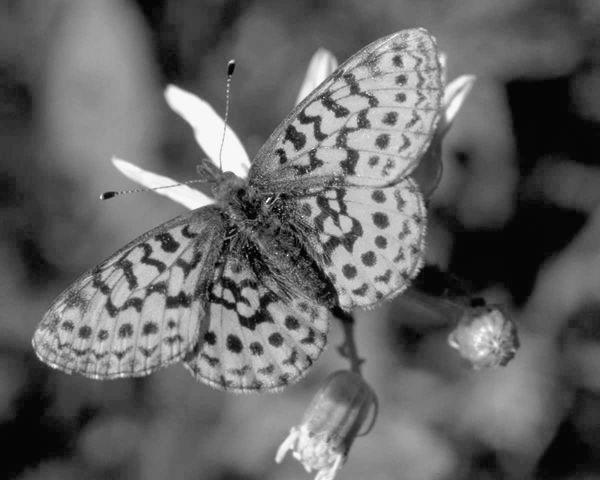
\includegraphics[scale=.3]{edge/butterfly.jpg}}
\quad
\subfloat[][Sobel]{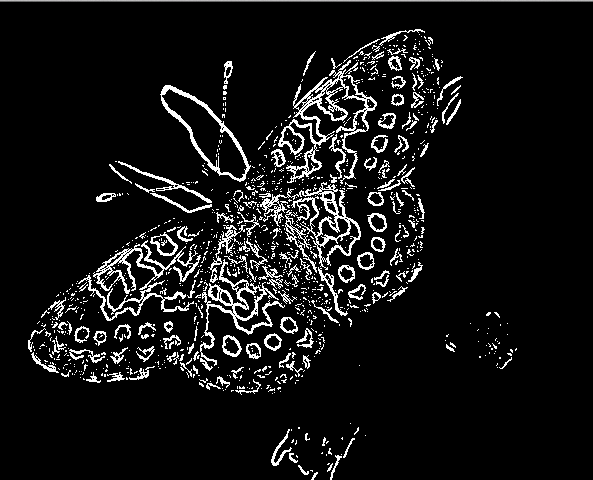
\includegraphics[scale=.3]{edge/sobel_butterfly.png}}
\quad
\subfloat[][Canny]{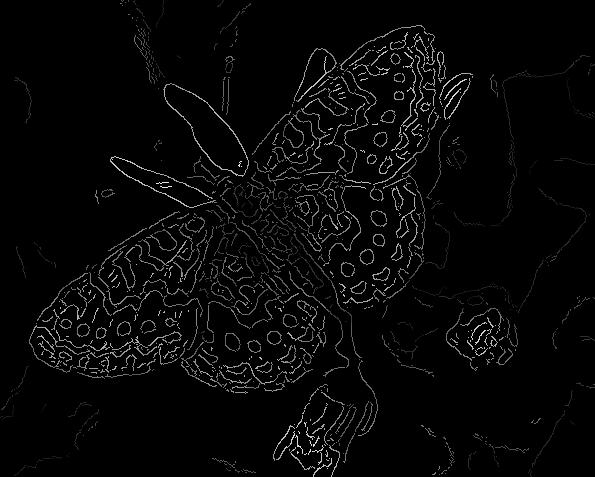
\includegraphics[scale=.3]{edge/canny_butterfly.png}}
\quad

\caption{Butterfly}%
\label{fig:a1b}%
\end{figure}

\begin{figure}%
\centering
\subfloat[][Original Image]{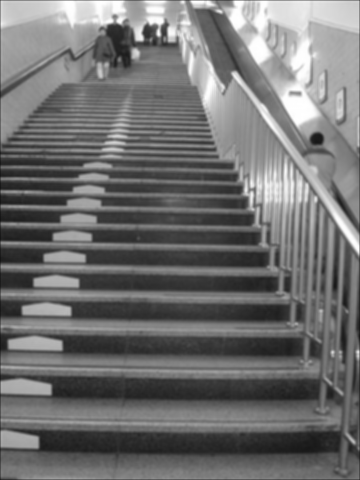
\includegraphics[scale=.4]{edge/stairs.png}}
\quad
\subfloat[][Sobel]{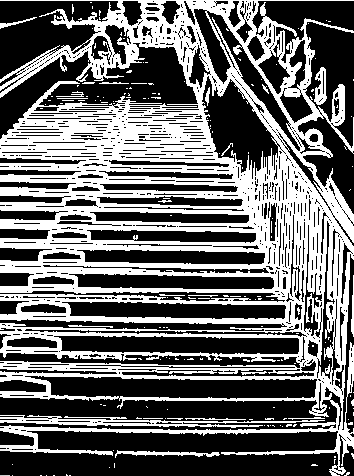
\includegraphics[scale=.4]{edge/sobel_stairs.png}}
\quad
\subfloat[][Canny. In the original sized image, edges are visible more clearly.]{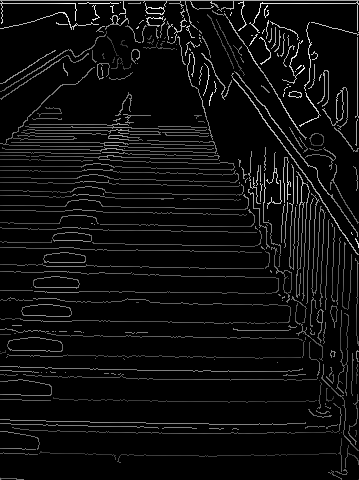
\includegraphics[scale=.4]{edge/canny_stairs.png}}
\quad

\caption{Stairs}%
\label{fig:a1b}%
\end{figure}

\begin{figure}%
\centering
\subfloat[][Original Image]{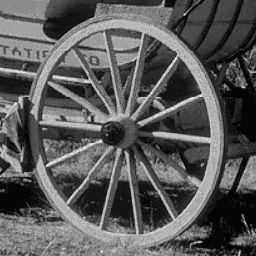
\includegraphics[scale=1]{edge/wheel.png}}
\quad
\subfloat[][Sobel]{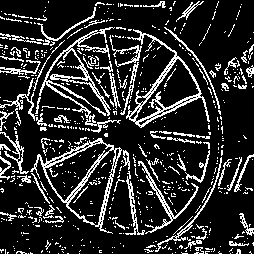
\includegraphics[scale=.4]{edge/sobel_wheel.png}}
\quad
\subfloat[][Canny.]{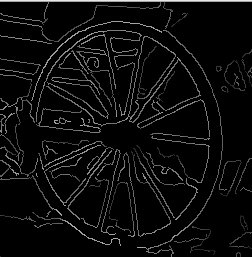
\includegraphics[scale=.4]{edge/canny_wheel.png}}
\quad

\caption{Wheel}%

\end{figure}

\begin{figure}%
\centering
\subfloat[][Original Image]{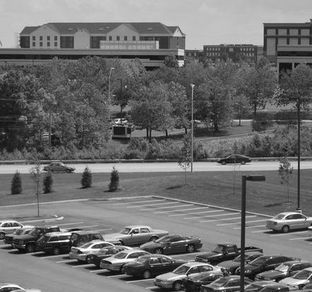
\includegraphics[scale=.4]{edge/outdoor.jpg}}
\quad
\subfloat[][Sobel]{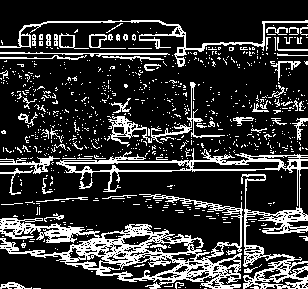
\includegraphics[scale=.4]{edge/sobel_outdoor.png}}
\quad
\subfloat[][Canny.]{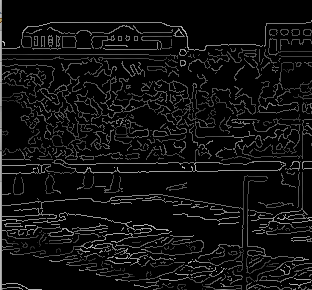
\includegraphics[scale=.4]{edge/canny_outdoor.png}}
\quad

\caption{Outdoor}%

\end{figure}

\begin{figure}%
\centering
\subfloat[][Original Image]{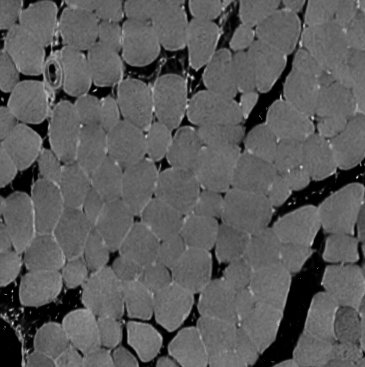
\includegraphics[scale=.4]{edge/cells.jpg}}
\quad
\subfloat[][Sobel]{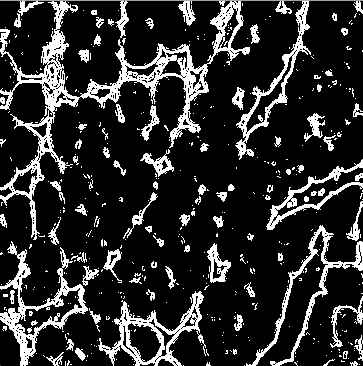
\includegraphics[scale=.4]{edge/sobel_cells.png}}
\quad
\subfloat[][Canny.]{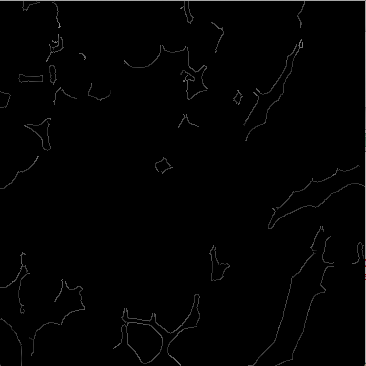
\includegraphics[scale=.4]{edge/canny_cells.png}}
\quad

\caption{Cells}%

\end{figure}


\subsection{Comparison}


Canny Edge detector lets you set more parameters, this can be useful, but it usually also takes longer to find an optimal combination of the different parameters. Canny edge detector seems more robust than the sobel one, additionally edges are only 1px thick, allowing clear localization of the edge.  I would always prefer the canny edge detector over the sobel edge detector, since at the heart of the canny edge detector lies a sobel operation. However, with the hysteresis thresholding, the canny edge detector tries to make edges more continuous. Although finding an optimal set of parameters can be tedious, I guess once it is found for a particular picture, it can be reapplied to similar pictures (i.e. pictures taken under the same conditions).  In general, edge detection is a very complex problem, especially in complex scenes. Even for us it is sometimes hard to judge in pictures such as cells.jpg where the true edges are. Additionally sometimes we don't want to detect all the edges, but only a subset of them. Also, for us humans equipped with stereo vision, we know at leas to basic classes of edges which are fundamentally different: texture edges (such as black paint on white paper) and spatial edges (edge of table,...). In a 2D image, this distinction cannot be made.



\FloatBarrier

\section{Hough transformation}
\subsection{Step size}
We have compared the results of the Hough transformation while varying different parameters.
For the parameter rho (Fig. \ref{fig:a2b}), we have discovered that making it too large will result in some lines being "overlooked", as the big step sizes simply step over the direction of a line. For theta (Fig. \ref{fig:a2a}), a larger value will discover more lines. This is, because when more finely grained, votes for the same line in the image will be distributed among neighboring accumulator cells, where as when coarsly grained, a single accumulator cell might indicate multiple similar lines. For the number of votes needed to be classified as a line (Fig. \ref{fig:a2c}), we obtained the intuitive result of getting more lines, the less votes are needed.


\begin{figure}%
\centering
\subfloat[][Rho = 0.5\degree]{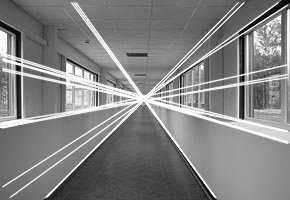
\includegraphics[scale=.3]{hough/res/corridorr0_5.jpg}}
\quad
\subfloat[][Rho = 1.0\degree]{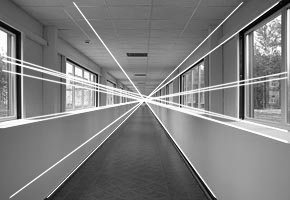
\includegraphics[scale=.3]{hough/res/corridor.jpg}}
\quad
\subfloat[][Rho = 2.0\degree]{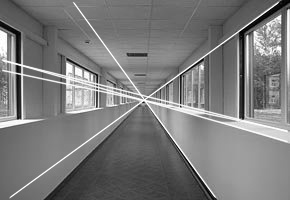
\includegraphics[scale=.3]{hough/res/corridorr2.jpg}}
\quad
\caption{Hough transform for detecting lines with varying rho.}%
\label{fig:a2b}%
\end{figure}

\begin{figure}%
\centering
\subfloat[][Theta = 0.5]{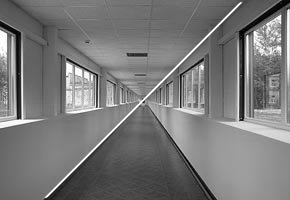
\includegraphics[scale=.3]{hough/res/corridort0_5.jpg}}
\quad
\subfloat[][Theta = 1.0]{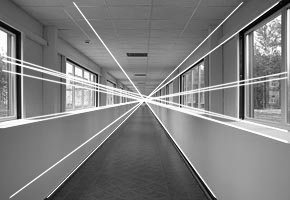
\includegraphics[scale=.3]{hough/res/corridor.jpg}}
\quad
\subfloat[][Theta = 2.0]{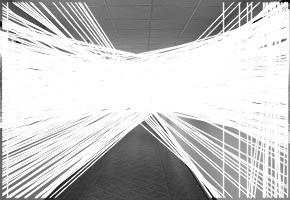
\includegraphics[scale=.3]{hough/res/corridort2.jpg}}
\quad
\caption{Hough transform for detecting lines with varying theta.}%
\label{fig:a2a}%
\end{figure}

\begin{figure}%
\centering
\subfloat[][N = 80]{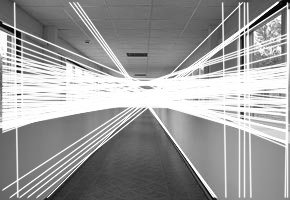
\includegraphics[scale=.3]{hough/res/corridorn80.jpg}}
\quad
\subfloat[][N = 100]{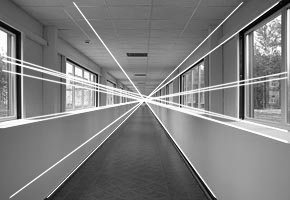
\includegraphics[scale=.3]{hough/res/corridor.jpg}}
\quad
\subfloat[][N = 120]{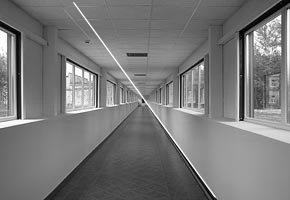
\includegraphics[scale=.3]{hough/res/corridorn120.jpg}}
\quad
\caption{Hough transform for detecting lines with varying number of votes N needed to be classified as line.}%
\label{fig:a2c}%
\end{figure}

\subsection{Line detection}
Here, we have summarized our results in Fig. \ref{fig:a2d} with tuned parameters.

\begin{figure}%
\centering
\subfloat[][theta=1,rho=1\degree,N=100]{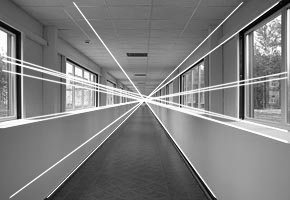
\includegraphics[scale=.3]{hough/res/corridor.jpg}}
\quad
\subfloat[][theta=3/4,rho=3/4\degree,N=140]{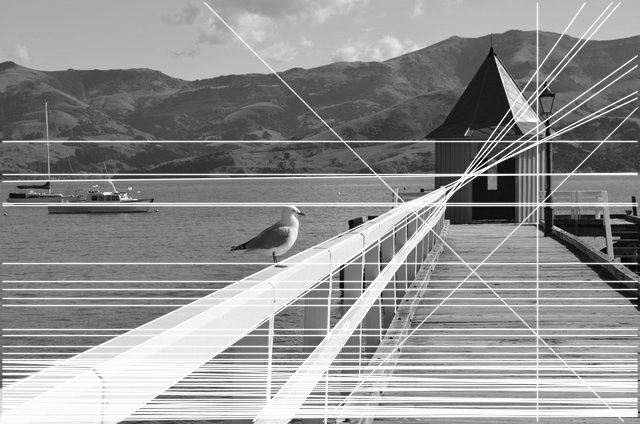
\includegraphics[scale=.3]{hough/res/outdoor.jpg}}
\quad
\subfloat[][theta=3/4,rho=3/4\degree,N=77]{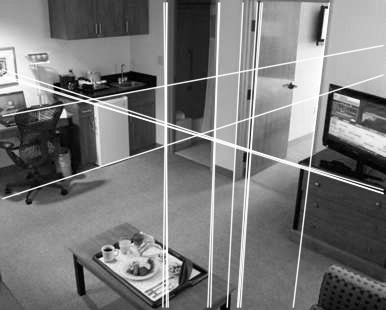
\includegraphics[scale=.3]{hough/res/room_1.jpg}}
\quad
\subfloat[][theta=3/4,rho=3/4\degree,N=105]{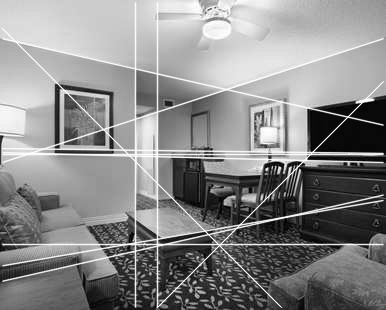
\includegraphics[scale=.3]{hough/res/room_2.jpg}}
\quad
\subfloat[][theta=1,rho=1\degree,N=130]{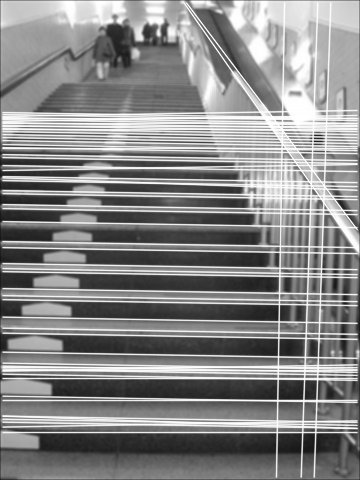
\includegraphics[scale=.3]{hough/res/stairs.png}}
\quad
\caption{Line detection with Hough, preprocessed with Canny}%
\label{fig:a2d}%
\end{figure}

\subsection{Complexity}
Since the algorithm has to test for every combination of rho and theta, the complexity is proportional to the number of rhos times the number of thetas.

\subsection{Multiple lines detected}
Our approach to solving the propblem of multiple similar lines being detected for the same line in the image is a rather simple one. Since these similar lines lie closely together in the hough accumulator (mostly neighboring cells), we need a way to combine clusters of high valued cells. We would do this by blurring the image, for example by convolving with a gauss kernel and then either apply a threshold function to the accumulator or subsample the accumulator to halve it in size. Repetition of this should eliminate the double-detection of the same lines.

\subsection{HoughLinesP}
We have tried out the HoughLinesP function with the same parameters as above, except that we adjusted the number of votes needed to 1/3rd of the above numbers. We have discovered that this function is better at finding also short lines. The results can be seen in Fig. \ref{fig:a2e}

\begin{figure}%
\centering
\subfloat[][theta=1,rho=1\degree,N=33]{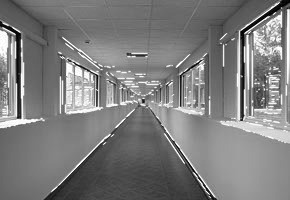
\includegraphics[scale=.3]{hough/res/Pcorridor.jpg}}
\quad
\subfloat[][theta=3/4,rho=3/4\degree,N=46]{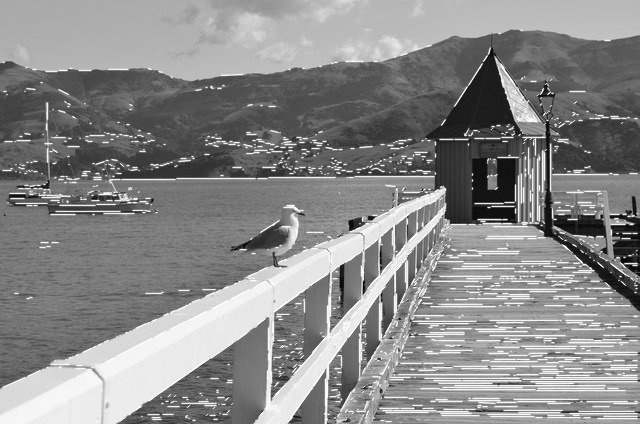
\includegraphics[scale=.3]{hough/res/Poutdoor.jpg}}
\quad
\subfloat[][theta=3/4,rho=3/4\degree,N=25]{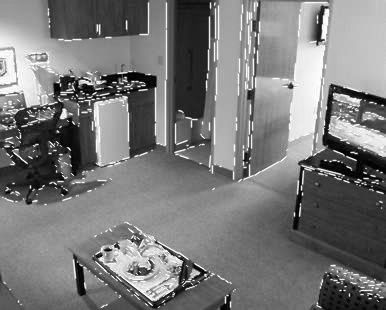
\includegraphics[scale=.3]{hough/res/Proom_1.jpg}}
\quad
\subfloat[][theta=3/4,rho=3/4\degree,N=35]{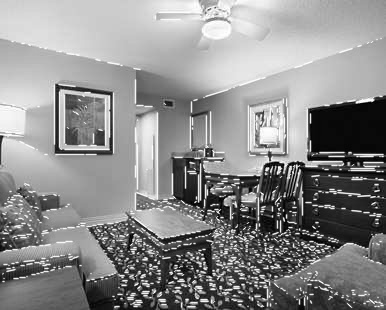
\includegraphics[scale=.3]{hough/res/Proom_2.jpg}}
\quad
\subfloat[][theta=1,rho=1\degree,N=43]{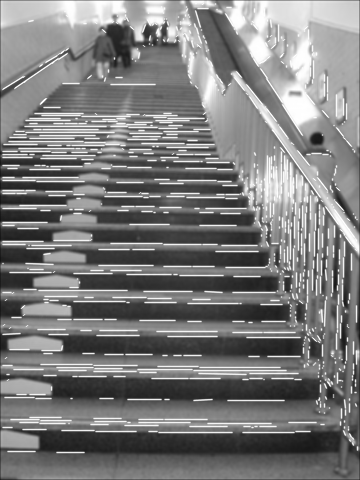
\includegraphics[scale=.3]{hough/res/Pstairs.png}}
\quad
\caption{Line detection with HoughLinesP, preprocessed with Canny}%
\label{fig:a2e}%
\end{figure}


\end{document}
